\task{Разрезания и углы}
\begin{itemize}

\itA Разрежьте тупоугольный треугольник ниже на семь остроугольных треугольников. Прямоугольный треугольник не считается остро-\linebreak угольным.

\begin{center}
	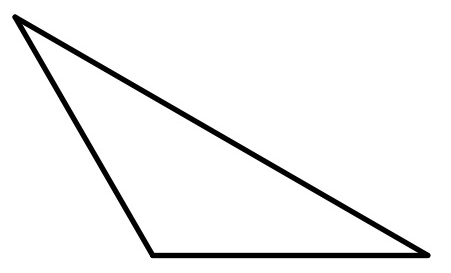
\includegraphics[width=3.6cm]{stats/2017/images/z_obtuse.png}
\end{center}

\itB Дан квадрат со стороной \SI{1}{\text{см}}. Покажите, как разрезать его на остроугольные треугольники.

\itC Докажите, что сумма величин углов $A$ и $B$ на рисунке равна величине угла $C$.

\begin{center}
	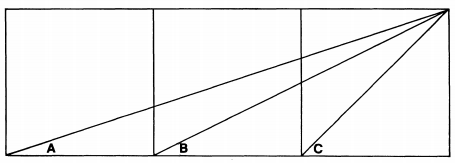
\includegraphics[width=8cm]{stats/2017/images/z_threesquares.png}
\end{center}
\end{itemize}